\chapter{Methods, data and evaluation}
\label{chapter:Methods}

%describe in detail architecture of the tencent MPNN and its variants, optionally discuss the code explain where the code is found and how to run it

\section{Data}
\label{sec:data-and-features}


\subsection{The CHAMPS dataset}
\label{sec:champs-dataset}

% TODO add dataset stats

Target variable is a magnetic interaction between two atoms measured by Nuclear Magnetic Resonance (NMR) - the scalar coupling constant or J-coupling constant~\cite{NMR}.
Note that in the graph notation, this is an edge-property as described in Section~\ref{sec:graph-output}. This interaction does not have to be predicted for any two atoms in the molecule but rather for a per-defined set of atom-pairs. These can be directly bonded to each other or be two or three covalent bonds apart. Furthermore, the can involve different atom types. The interactions are categorized into eight categories by the involved atom types and the number of bonds between them. For instance, $2JHC$ is the J-coupling type of a hydrogen- and a carbon-atom with two bonds between them. For a more detailed investigation, please follow the links to two Kaggle-notebooks in the footnotes~\footnote{\url{https://www.kaggle.com/rpeer333/molecular-properties-detailed-eda}}
~\footnote{\url{https://www.kaggle.com/rpeer333/champs-competition-baseline-trivial-predictions}}.
In a general model, this category would be the most important basic feature as the ranges of J-coupling constants differ markedly between those categories. However, another approach is to simply train a different model for each type. This approach has been shown to be effective with boosted tree-models as well as MPNNs and was therefore used in both cases.

% TODO describe quatratic kappa

\subsection{The \textit{Alchemy} dataset}
\label{sec:alchemy-dataset}
The new quantum chemistry dataset \textit{Alchemy}, created by Tencent Quantum Lab, was used for this thesis~\cite{Chen2019}. The dataset is similar to the well established QM9 dataset~\cite{Ramakrishnan2014} with the same quantum mechanical properties available and a similar number of molecules. The main advantage of the new \textit{Alchemy} dataset is that it also contains larger molecules of up to 14 heavy atoms (i.e. non-hydrogen atoms) as opposed to the maximum of nine heavy atoms in the QM9 dataset. This property makes it more relevant for medically oriented research as potential drugs are not limited to only very small molecules. 
There 119487 molecules in the dataset containing the 3D coordinates for each atom, its type and the information which atoms are covalently bonded with which bond type and twelve important quantum mechanical properties~\cite{Chen2019} of the molecule~\footnote{
	Unfortunately, due to the issue described in Section~\ref{sec:diff-old-new-ds}, the test set could not be used for reliable evaluation. The remaining dataset consists of 99776 molecules in the training-set and 3951 molecules in the validation set.
}. The task is to predict those twelve properties~\footnote{
	The 12 target variables
	(Dipole moment, Polarizability, HOMO, LUMO, gap, R\textsuperscript2, Zero point energy, Internal energy, Internal energy at 298.15 K, Enthalpy at 298.15 K, Free energy at 298.15 K, Heat capacity at 298.15 K) are shown in Table~2 of Chen et. al.~\cite{Chen2019}.
} from the raw data. The target properties have been calculated using computationally highly expensive quantum chemical computations using the python library \textit{PySCF}~\cite{Sun2017}.



\subsection{Features}
\label{sec:features}

There are two different approaches to go about the task. The pure deep learning approach is to use only coordinates and bonds and rely on the network to learn any features required to predict the target properties. After all, coordinates, atom types and bonds contain all the available information (actually the bonds could be reliably calculated from coordinates and atom types and thus, strictly speaking are also redundant information).

The other approach is to calculate all sorts of chemical features using chemistry python libraries and feed them in to the model alongside the raw data. These include node (atom) features (whether the atom is an electron donor or acceptor, whether it is part of an aromatic ring, it's hybridization type, etc.~\cite{Organic-chemistry}) as well as bond (edge) features. The fact that these features are calculated from the raw data without any additional information means that the model should also be able to learn to compute them if required. Hence, calculating features and feeding them into the model should in theory be obsolete but could slightly improve predictions if the model is unable to learn those features. Since the focus of this thesis is deep-learning, no manual feature computation is performed here except if it is required to allow comparison with results from the literature.


\section{Model architecture}
\label{sec:architecture}

\subsection{\textit{SchNet}}
\label{sec:schnet-architecture}

As this model has not been used for many experiments, we shall refer to the literature instead. The implementation follows the architecture proposed by Schütt et. al.~\cite{Schutt2017}. Several changes were made in the DGL-implementation~\footnote{\url{https://www.kaggle.com/rpeer333/pytorch-dgl-schnet-a-graph-convolutional-net}} compared to the template \textit{Chainer}-implementation~\footnote{\url{https://www.kaggle.com/toshik/schnet-starter-kit}}. In particular, a graph state was added. This is similar to the concept of a root- or master-node shown in Section~\ref{sec:root-node}. Furthermore the residual short-cuts (first used in \textit{ResNets}~\cite{Sun2016}) in the graph convolution layers were replaced with dense short cuts analogous to the ones form \textit{DenseNets}~\cite{Huang2017}. Neither of those changes is responsible for the poor performance of the model as the results were the same with them.


\subsection{Base MPNN architecture}
\label{sec:mpnn-architecture}

The basic architecture used as a starting point for most of the experiments in this thesis (Section~\ref{sec:alchemy}) comes from the MPNN variant from Chen et. al.~\cite{Chen2019} whose code is available on GitHub~\footnote{\url{https://github.com/tencent-alchemy/Alchemy}}. This model, in turn is based on the MPNN model proposed by Gilmer et. al.~\cite{Gilmer2017}.


\paragraph{Node embedding}The networks starts with an embedding of the atom-type of each node. In this particular implementation, this is achieved by passing a the one-hot encoded atom type through a regular linear layer. This first layer essentially extracts the n\textsuperscript{nt} column from the weight matrix when the n\textsuperscript{th} position of the input vector is one which is easy to see from the following example.

\begin{equation}
\begin{bmatrix} 
w_{11} & w_{12} & w_{13} \\
w_{21} & w_{22} & w_{23} \\
w_{31} & w_{32} & w_{33} \\
\end{bmatrix}
*
\begin{bmatrix} 
1 \\
0 \\
0 \\
\end{bmatrix}
=
\begin{bmatrix} 
w_{11} \\
w_{21} \\
w_{31} \\
\end{bmatrix}
\end{equation}

Thus, the first linear layer essentially corresponds to a mapping from a categorical, integer-valued variable to vector $\in \mathbb{R}^d$ where $d$ is the output dimension of the linear layer which defines the dimension of the node hidden state.

\paragraph{Message passing}

The message passing function used in the experiments was the so called edge network message function which was found to be the best among several options by Gilmer et. al.~\cite{Gilmer2017}. The approach is described in more detail and nicely illustrated by Simonovsky et. at.~\cite{Simonovsky2017}. This message passing layer is implemented in the \textit{PyTorch Geometric} class NNConv~\footnote{\url{https://pytorch-geometric.readthedocs.io/en/latest/modules/nn.html}}\label{fn:pytorch-geometric-nn-docs}.


The message function has two components. The first one is a two-layer MLP (multi-layer perceptron)  $h_{\mathbf{\Theta}}$ taking the edge features as input and putting out a vector of dimension $d^2$ which is reshaped into a $d$ by $d$ matrix.

\begin{equation}
	\Theta_{vw} = reshape(~h_{\Theta}(e_{vw})~)
\end{equation}

In the second step, the sending node representation $h_j$ is multiplied with this edge-conditioned weight matrix. Finally, an aggregation over all sending (neighboring) nodes gives the message for node $w$.

\begin{equation}
 m_v^{t+1} = \sum_{w \in \mathcal{N}(v)} h_w^t \cdot \Theta_{vw}
\end{equation}

It is easy to see how the two functions can be combined in a single message-function. Finally, in the default setting, the update function is simply

\begin{equation}
	h_v^{t+1} = m_v^{t+1}
\end{equation}
\label{eq:update-nnconv-simple}

If the root-node concept is used (by setting the parameter root-weight to 'True')\footnote{
	Technically, as Equation~\ref{eq:update-nnconv-root} shows, there is no root-node in this architecture. There is just the root weight-matrix $\Theta_{root}$ which can be thought of as a representation of an edge between the virtual root node and any real node in the graph. However, that is just an implementation detail which depends on this particular architecture. It is still valid to see $\Theta_{root}$ as the concept of a root node which can be extended to other architectures as well - just implemented differently.
} the update function becomes

\begin{equation}
h_v^{t+1} = \Theta_{root}h_v^t~+~m_v^{t+1}
\end{equation}

\label{eq:update-nnconv-root}


Oddly enough, in the simple case of Equation~\ref{eq:update-nnconv-simple}, the updated node hidden state $h_v^{t+1}$ is not a function of the previous hidden state $h_v^t$. While that is counter-intuitive, it was shown to work well in practice. Section~\ref{sec:root-node} compares the same mode with and without the root-node and finds no difference in performance.

\paragraph{Readout function} Finally, the readout function is composed of a \textit{Set2Set} (also documented in the link of Footnote~\ref{fn:pytorch-geometric-nn-docs}) layer mapping the set of node hidden states to an aggregated representation. Then, the output from \textit{Set2Set} is mapped to the target variable with a two-layer MLP. The readout-function can be formalized as

\begin{equation}
		\hat{y} = MLP(~Set2Set(~\{h_v^T\ | v \in G~\})~)
\end{equation}

\section{Software}

Most of the models presented in this thesis (Section~\ref{sec:alchemy}) were implemented using the python deep learning library \textit{PyTorch}~\footnote{\url{https://pytorch.org/}} and its extension for graph neural networks, \textit{PyTorch Geometric}~\footnote{\url{https://pytorch-geometric.readthedocs.io/en/latest/}}. The \textit{SchNet} model (Section~\ref{sec:schnet}) was implemented using the python library DGL (deep graph library)~\footnote{\url{https://www.dgl.ai/}}. In my humble opinion, \textit{PyTorch Geometric} is by far superior to DGL. It's API is much more in line with \textit{PyTorch}, the documentation is clear and the code works reliably. On the other hand, DGL is not easy to use and the work on the \textit{SchNet} model was severely hampered by a memory leak: the GPU memory filled-up over time and not released again. In order to fix this issue, all caches have to be cleared after each batch leading extremely slow training making it impossible to try different approaches in limited time. Summing up, \textit{PyTorch Geometric} is the best \textit{PyTorch} compatible library for MPNN I have come across during the work for this thesis.

The code of the models trained on the \textit{Alchemy} dataset is available at github: \url{https://github.com/raph333/masters\_project}.



\section{Training}
\label{sec:training}

All experiments presented in this thesis use Adaptive Moment Estimation (Adam) for gradient descent~\cite{Kingma2015}. For certain experiments, other optimizers might give slightly better results. However, comparison between differences in data processing and network architectures would be impeded by employing different optimization schemes because one would never know if the different outcomes are a result of the model or the optimization. For this reason, optimization strategies were kept as constant as possible for all experiments.

The same considerations were applied to learning rates and learning rate scheduling. Two different optimization schemes were used for different purposes.
To obtain the lowest possible test-set error, a learning rate schedule that reduces the learning rate after the validation error plateaus has found to be most effective~\footnote{Specifically, the following parameters were chosen: The initial learning rate of 0.01 is reduced by a factor of 0.75 if the validation error did not decrease by a value of $10^{-4}$ or more within the last 10 epochs. The training duration was 300 epochs} This optimization scheme above suffers from the drawback of requiring many training epochs. Furthermore, the resulting learning-rate schedule varies considerably even between trainings with the same parameters. These differences as well as the long training time make it unsuitable for comparing learning curves with different parameters.
For comparing different learning curves a simpler, exponential learning-rate decay was chosen~\footnote{The initial learning rate of 0.001 is reduced by a factor of 0.995 after every epoch and the experiment is run for 150.} [CITATON]. The advantage of this method is that at each epoch, all curves have the same learning rate which makes them comparable. The final validation error is usually higher than would be achieved with reduce-on-plateau learning rate scheduling. However, this drawback is accepted because the main point of the experiments is to compare different model architectures, parameters or data-transformation rather than to achieve the lowest possible test-set error.


\section{Benchmark and evaluation}

The target variable in this dataset is a real-valued vector of length twelve. The error-metric used throughout this work is the mean absolute error (MAE) - which was also the metric in the Alchemy Contest. As the twelve quantum mechanical properties have vastly different ranges, they have to be normalized - otherwise the properties with larger ranges would contribute far more to the MAE than the properties with smaller ranges. Normalization was performed by subtracting the mean and dividing by the standard deviation.

\section{Difference between competition-dataset and full-dataset}
\label{sec:diff-old-new-ds}

%This subsection explains why the MAE-values presented in this thesis cannot be compared the competition leader-board including my own score with rank 26.

\paragraph{Overview} Unfortunately, the results obtained on the competition dataset cannot be directly compared to results achieved on the full dataset published after the competition. This section presents the result of an investigation in to the data quality issues and explains why the test-set (in particular the target variables) could not be used for the experiments. If the reader is only interested in the main topic of the theses rather then the inconsistencies in the particular dataset chosen for the experiments, this subsection may be skipped. On the other hand, if the reader intends to train a model on this dataset then reading through this section can save a lot of time.

Figure~\ref{fig:competition-vs-full-ds} shows the learning curves of models being trained on both the competition-dataset and the full dataset. The MAE values are considerably lower on the competition dataset.


\begin{figure}[H]
	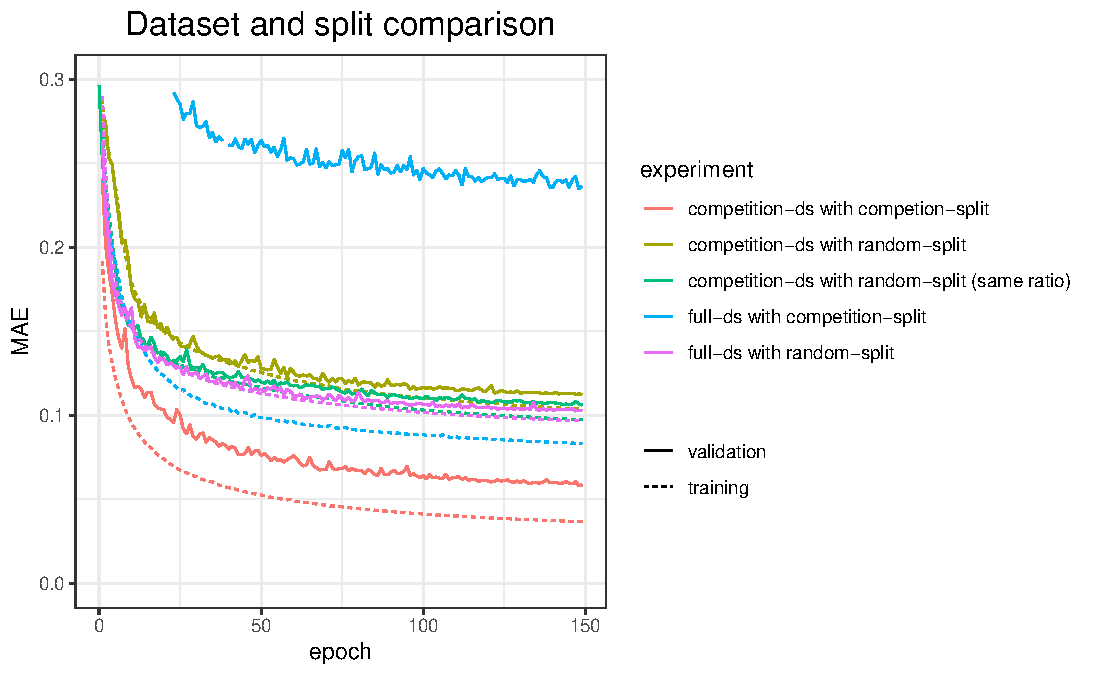
\includegraphics[width=\linewidth]{figures/competition-vs-full-ds}
	\caption{Comparing the full (post-competition) and the competition dataset using various methods for splitting the data into training- and validation-set. Both data-sets are evaluated using a random split (70\% training, 15\% validation, 15\% testing) and the train-validation split as it was defined in the competition (bias towards higher weight molecules in the validation set). In addition, the competition data is also subjected to a random split where the fraction of the validation-set is exactly the same as in the competition-data-split. (This last experiment was conducted to make sure that the observed difference is due to the method of splitting and not due to the size of the validation set.)}
	\label{fig:competition-vs-full-ds}
\end{figure}

\paragraph{Train-test split}
The competition data-set is split into training-set (called dev-set by the competition hosts), validation- and test-set with the ground truth being provided only for the first two sets. The split is not random. Instead, the validation- and test-set have an intentional bias towards larger molecules compared to the training-set. Building models that can extrapolate from smaller molecules to larger molecules is useful for pharmacological research~\cite{Chen2019}.
%However, in order to focus on the core topic of GCNN for molecules, for most experiments presented in this thesis. I only use a simple random split where training-, validation- and test-set are randomly drawn without replacement from the same population.

Figure~\ref{fig:competition-vs-full-ds} shows learning curves for both competition-data split and random split to eliminate any differences in validation MAE hailing from the different dataset splits.
The figure shows two counterintuitive results. First of all, the MAE on is higher on the full dataset despite it's larger size. Naturally the larger dataset should give better or at least equally good results. Secondly, the impact of the splitting method varies between the two dataset. The expected result would have been a lower MAE on randomly split data because the training- and validation- molecules come from the same distribution. Having a strong bias towards higher weight molecules in the validation set is expected to increase the MAE. For the full dataset, this is indeed the case. However, for the competition dataset, the random split gives a higher MAE than the biased competition split. As this result contradicts the expectation, it was heavily tested and validated.

%First of all, it is obvious that the validation MAE is lower on the randomly split data. This comes as no surprise because in the competition-data split, the validation molecules are systematically different (larger) from the training molecules. However, regardless of the kind of data-split, the MAE-values are still consistently lower on the competition data.


\paragraph{Target variable normalization}

In the competition data-set, the values are already normalized and the raw values are not available. It is not clear whether the mean and standard deviation used for normalization where calculated separately for the training- and validation-set or if the they are based on all molecules. Furthermore, the order of the target variables is unknown (by design) and their names are replaced with the dummy-names property-1, property-2, etc.

The full dataset released after the competition contains the raw values and the real names of the target variables. For training and evaluation, they were normalized in the same manner as in the competition (subtraction of mean and division by standard deviation). However, a direct comparison with the ranges of the competition dataset is not possible as the names of the target variables are not provided there. 

The only observation that can be made is that the average range (maximum - minimum) of all target variables is lower in the competition data-set. This suggest that the normalization might have been conducted on per-set basis because the range within a subset of the data is necessarily smaller or equal than the range of the full dataset. However, the small difference of an average range of 8.66 in the competition dataset and 9.72 in the full dataset is insufficient to explain the difference in MAE between the two datasets. Furthermore, such a difference could just as well be a function of dataset-size as larger datasets have a higher probability of containing more extreme outliers which increases the range of the target variables.

\paragraph{Molecule data}

The raw data and thus the input into the model is exactly the same in the full dataset as in the competition dataset. This has been thoroughly tested and verified.

\paragraph{Conclusion}

With the input-data as well as the data-splits being identical, the reason for the difference in MAE can only be explained by the different values of the target variables. As discussed above, the absence of raw data in the competition dataset prevents a direct comparison of the target variables between the two datasets. Thus, no further information can be obtained to pinpoint the difference or to find a possible explanation. The only conclusion to be made is that for some reason the target variables in the new data prevent the net from learning to predict them as well as in the competition data. For this reason, I chose to use the labeled competition data for the experiments in this thesis. This comprises 103727 molecules from the training- and validation-set of the competition data.
Furthermore, I chose use the same training-validation split as in the competition because the MAE of the competition-data with this split could not be achieved by any other splitting method. While it is unfortunate not to know the root of this counterintuitive finding, it will have to remain a mystery in order to focus on the core topic of this thesis: graph neural networks. 

 
\section{Experiments}

Most experiments show learning curves with validation- and training-error rather than just the final errors. The choice was made because, in addition to showing the final error-rates, learning curves allow to estimate whether the model suffers from high bias or high variance and also shows if prolonged training could lead to further improvements or if a plateau has been reached. In contrast, a single error-metric does not show how this metric was obtained and thus offers little information to interpret the results. Furthermore, learning curve averaging of multiple training runs was employed to reduce the impact of noise. Some variation in the learning curves is to be expected even in the absence of any difference in model architecture, input data or optimization strategy. Therefore, any given learning curve shown in this thesis is an average of three independent learning curves using the exact same models parameters and input data. Conduction multiple training runs for each setting and averaging the results reduces the impact of random variation and allow to see the systematic differences instead. 

% appendix: interpreting learning curves

